\section{Differential drive}

The differential drive robot consists of two wheels positioned on the same axis, each with its own independent motor, along with a third passive supporting wheel.
\begin{figure}[H]
    \centering
    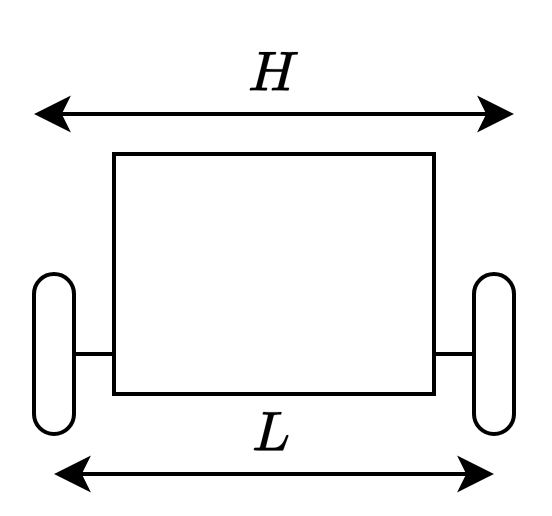
\includegraphics[width=0.25\linewidth]{images/ddk.png} 
    \caption{Differential drive robot}
\end{figure}
The baseline $L$ represents the distance between the contact points of the wheels.

The variables under independent control are the velocities of the right wheel, $v_R$, and the left wheel, $v_L$. 
The robot's pose is represented in the base reference frame as $P(x, y, \theta)$.

Control inputs are the linear velocity of the robot, $v$, and its angular velocity, $\omega$, which are linearly related to $v_R$ and $v_L$. 
Both right and left wheels follow circular paths with an angular velocity of $\omega$ and different curvature radii $R$:
\[\begin{cases}
    \omega\left(R+\frac{L}{2}\right)=v_R \\
    \omega\left(R+\frac{L}{2}\right)=v_L \\
\end{cases}\]
Given $v_R$ and $v_L$, $\omega$ can be found by solving for $R$ and equating:
\[\omega =\dfrac{ v_R - v_L}{L}\]
Similarly, $R$ can be found by solving for $\omega$ and equating:
\[R=\dfrac{L}{2}\dfrac{v_R+v_L}{v_R-v_L}\]
Note that rotation in place is achieved by setting $R=0$ and $v_R=-v_L$, while linear movement is accomplished by setting $T=\infty$ and $v_R=v_L$.

The wheels move around an Instantaneous Center of Curvature (ICC) on a circumference with an instantaneous radius $R$ and angular velocity $\omega$:
\[\text{ICC}=\left\{ x+R\cos\left(\theta+\dfrac{\pi}{2}\right), y+R\sin\left(\theta+\dfrac{\pi}{2}\right) \right\}=\left\{ x-R\sin\left(\theta\right), y+R\cos\left(\theta\right) \right\}\]

The overall change in position over time is given by the equation:
\[\begin{bmatrix}
    x^\prime \\ 
    y^\prime \\
    \theta^\prime
\end{bmatrix} = 
\begin{bmatrix}
    \cos(\omega \cdot \delta t) & -\sin(\omega \cdot \delta t) & 0 \\
    \sin(\omega \cdot \delta t) & \cos(\omega \cdot \delta t) & 0 \\
    0 & 0 & 1
\end{bmatrix} \begin{bmatrix}
    x-\text{ICC}_x \\
    y-\text{ICC}_y \\
    \theta
\end{bmatrix} + \begin{bmatrix}
    \text{ICC}_x \\
    \text{ICC}_y \\
    \omega \cdot \delta t
\end{bmatrix}\]
Finally, the control inputs are defined by the following formulas:
\[v=\dfrac{v_R+v_L}{2} \qquad \omega =\dfrac{v_R-v_L}{L}\]
Where a positive angular velocity indicates the robot is turning left, otherwise it turns right. 
Additionally, when velocities are equal, the robot exhibits lower angular velocity if $L$ is large, and higher otherwise.

\subsection{Odometry}
Given the known angular speed $\omega$, the radius of the Instantaneous Center of Curvature (ICC) $R$, and the linear velocity $v$ at each time instant, we can reconstruct the path and the final trajectory.
This reconstruction of the path via integration is termed odometry.

The odometry of this robot involves computing the velocity in the base frame:
\[\begin{cases}
    v_x=v(t)\cos\left(\theta(t) \right) \\ 
    v_y=v(t)\sin\left(\theta(t) \right)
\end{cases}\]
Integrating the position in the base frame yields:
\[\begin{cases}
    x(t)=\int v(t)\cos\left(\theta(t) \right) \\
    y(t)=\int v(t)\sin\left(\theta(t) \right) \\
    \theta(t)=\int \omega(t) dt
\end{cases}\]
Considering the velocities of both wheels $v_R$ and $v_L$ at a discrete time $t^\prime$, we have:
\[\begin{cases}
    x(t)=\frac{1}{2} \int_0^t \left( v_R(t^\prime) + v_L(t^\prime) \right)\cos\left(\theta(t^\prime) \right) \\
    y(t)=\frac{1}{2} \int_0^t \left( v_R(t^\prime) + v_L(t^\prime) \right)\sin\left(\theta(t^\prime) \right) \\
    \theta(t)=\frac{1}{L} \int_0^t \left( v_R(t^\prime) - v_L(t^\prime) \right) dt^\prime
\end{cases}\]
Since computing these integrals is computationally intensive, we may resort to using approximations at discrete time instants.

\paragraph*{Euler's integration}
When assuming constant linear velocity $v_k$ and angular velocity $\omega_k$ within the time interval $\left[ t_k,t_{k+1} \right]$, Euler integration can be employed to compute the robot odometry:
\[\begin{cases}
    x_{k+1} = x_k + v_kT_S\cos\theta_k \\
    y_{k+1} = y_k + v_kT_S\sin\theta_k \\
    \theta_{k+1} = \theta_k + \omega_kT_S \\
    T_S=t_{k+1}-t_k
\end{cases}\]
Here, the position $\left\{x_{k+1}, y_{k+1}\right\}$ is approximated, while the angle $\theta_{k+1}$ remains exact.

\paragraph*{Runge-Kutta's integration}
Assuming constant linear velocity $v_k$ and angular velocity $\omega_k$ within the time interval $\left[ t_k,t_{k+1} \right]$, second-order Runge-Kutta integration can be used for computing robot odometry:
\[\begin{cases}
    x_{k+1} = x_k + v_kT_S\cos \left(\theta_k + \dfrac{\omega_kT_S}{2} \right)\\
    y_{k+1} = y_k + v_kT_S\sin\left(\theta_k + \dfrac{\omega_kT_S}{2} \right) \\
    \theta_{k+1} = \theta_k + \omega_kT_S \\
    T_S=t_{k+1}-t_k
\end{cases}\]
Although this method provides a better approximation, the orientation is not exact.

\paragraph*{Exact integration}
When assuming constant linear velocity $v_k$ and angular velocity $\omega_k$ within the time interval $\left[ t_k,t_{k+1} \right]$, exact integration can be utilized to compute the robot odometry, resulting in:
\[\begin{cases}
    x_{k+1} = x_k + \dfrac{v_k}{\omega_k}\left( \sin\theta_{k+1} - \sin\theta_k \right) \\
    y_{k+1} = y_k - \dfrac{v_k}{\omega_k}\left( \cos\theta_{k+1} - \cos\theta_k \right) \\
    \theta_{k+1} = \theta_k + \omega_kT_S \\
    T_S=t_{k+1}-t_k
\end{cases}\]
In this case, all measurements are exact, but special attention must be given when the robot travels straight ($\omega \sim 0$). 
In such cases, Runge-Kutta integration should be used.
\begin{figure}[H]
    \centering
    \begin{subfigure}{0.32\textwidth}
        \centering
        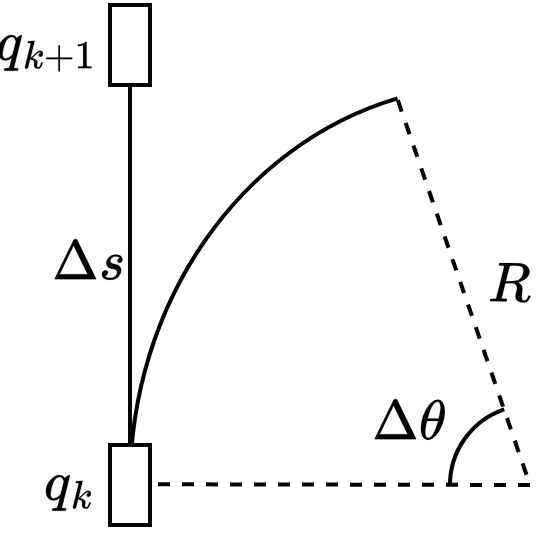
\includegraphics[width=0.6\linewidth]{images/euler.png} 
        \caption{Euler}
    \end{subfigure}
    \begin{subfigure}{0.32\textwidth}
        \centering
        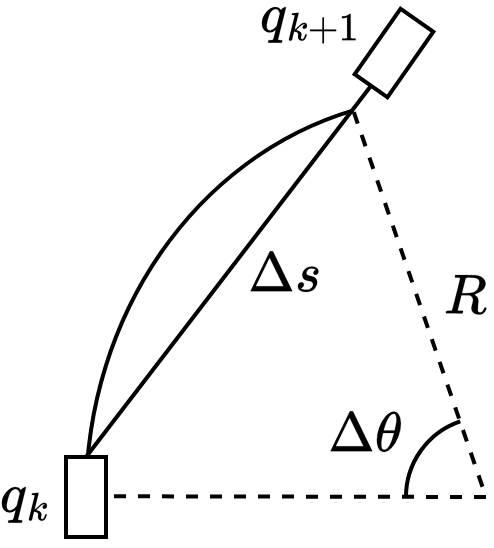
\includegraphics[width=0.6\linewidth]{images/rk.png}
        \caption{Runge-Kutta}
    \end{subfigure}
    \begin{subfigure}{0.32\textwidth}
        \centering
        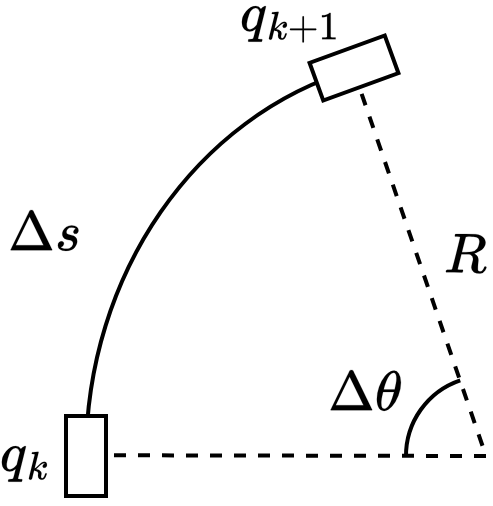
\includegraphics[width=0.6\linewidth]{images/exact.png}
        \caption{Exact}
    \end{subfigure}
    \caption{Integration techniques}
\end{figure}
These integration techniques serve different purposes depending on the system's frequency and the frequency at which parameters are checked. 
Euler and Runge-Kutta methods are suitable for high-frequency systems, while the exact approximation is necessary for low-frequency systems.

\subsection{Sensors}
Proprioceptive measurements are utilized to calculate linear velocity $v_k$ and angular velocity $\omega_k$:
\[\begin{cases}
    v_kT_S=\Delta s \\
    \omega_kT_S=\Delta\theta
\end{cases} \implies \dfrac{\Delta s}{\Delta\theta}=\dfrac{v_k}{\omega_k}\]
Here, $\Delta s$ represents the distance traveled and $\Delta\theta$ denotes the change in orientation.

In a differential drive system, these quantities become:
\[\Delta s=\dfrac{r}{2}\left(\Delta\phi_R+\Delta\phi_L\right) \qquad \Delta\theta=\dfrac{r}{L}\left(\Delta\phi_R-\Delta\phi_L\right)\]
Here, $\Delta\phi_R$ and $\Delta\phi_L$ correspond to the total rotations measured by wheel encoders.

It's important to note that this formula is applicable primarily for small-time frames, as larger ones introduce increased error due to various factors.